\documentclass[conference, a4paper]{IEEEtran}

\usepackage{cite}

\ifCLASSINFOpdf
  \usepackage[pdftex]{graphicx}
\else
  \usepackage[dvips]{graphicx}
\fi

\usepackage{url}
\usepackage{color}
\definecolor{tubafblue}{rgb}{0, 0.39215686274509803, 0.6588235294117647}
\definecolor{tubafgray}{rgb}{0.6039215686274509, 0.6078431372549019, 0.615686274509804}
\hyphenation{op-tical net-works semi-conduc-tor}




\begin{document}


\begin{titlepage}
	\vspace*{3mm}
	
	\hfill 
\includegraphics[width=75mm]{pics/WBM_eng_orig_RGB.jpg}

	\vspace*{5mm}


\hfill \begin{minipage}[t]{53mm}
	\resizebox{55mm}{!}{
	\begin{tabular}{l}
		\footnotesize{ {\color{tubafgray} \textsf{Faculty of Mathematics and Computer Science}}} \\
		\footnotesize{ {\color{tubafgray} \textsf{Institute of Computer Science}}} \\
		\footnotesize{ {\color{tubafgray} \textsf{Virtual Reality and Multimedia Group}}} \\
	\end{tabular}
	}
\end{minipage}

\begin{center}
  \vspace*{2.5cm}
	
  {\large \bf \textsf{Seminar paper}}\\

  \vspace*{1cm}
%
%
% TITEL DER ARBEIT
%
%
  {\color{tubafblue} \Huge \bf \textsf{Comparison of feature-based pose estimation and localization methods in dark environments}}\\  % HIER EINSETZEN!

  \vspace*{1cm}
%
%
% NAME DES STUDENTEN (auf Titelblatt)
%
% 
  {\Large \bf \textsf{Jonas Fleischer}}\\                  %
  % HIER EINSETZEN!

	\vspace*{7mm}
	{\large \textsf{Applied Computer Science}}\\  % HIER EINSETZEN!
	{\large \textsf{Specialization: Robotics}}\\  % HIER EINSETZEN!

  	\vspace*{10mm}
	{\large \textsf{Matriculation register: 61146}}\\  % HIER EINSETZEN!

  	\vspace*{1cm}
	{\large \textsf{August 30, 2024}}\\  % HIER EINSETZEN!

 
%  \vspace*{8cm}
%  {\Large \textsf{Seminar \emph{Cyber-Physical Systems} SoSe2015)}}\\
\end{center}	

\vfill

%
%
% NAME DES BETREUERS
%
%
	\noindent
    \hspace*{1cm}\textsf{Tutor/First Proofreader:}\\
    \hspace*{1cm}\textsf{Prof. Dr. Bernhard Jung}\\
    \\
	\noindent
    \hspace*{1cm}\textsf{Second Proofreader:}\\
    \hspace*{1cm}\textsf{Robert L{\"o}sch}\\
    \\
	\vspace*{-3cm}
\end{titlepage}


\title{Comparison of feature-based pose estimation and localization methods in dark environments}

\author{\IEEEauthorblockN{Jonas Fleischer}
\IEEEauthorblockA{Technische Universität Bergakademie Freiberg\\Fakultät für Mathematik und Informatik\\Institut für Informatik\\Bernhard-von-Cotta-Straße 2\\09599 Freiberg}}

\maketitle

\begin{abstract}
This paper presents a comparative analysis of feature-based pose estimation and localization methods, focusing on traditional algorithms such as Scale-Invariant Feature Transform (SIFT), Oriented FAST and Rotated BRIEF (ORB), and Accelerated-KAZE (AKAZE). These methods are crucial for autonomous navigation in environments where Global Navigation Satellite Systems (GNSS) are unreliable or unavailable, such as indoor settings. Additionally, the focus is on dark environments where no visual data is available. Therefore, depth images captured from sensors like LIDAR are intended to be used. To ensure reliability during testing, synthetic test data generated from sensors designed for low-light environments were utilized. However, due to implementation errors, the expected results were not fully realized. While the algorithms themselves are known for their robustness and accuracy, the limitations observed in this study stem from the current state of the implementation rather than the inherent capabilities of the algorithms. This work highlights the importance of careful implementation and testing, and it outlines the next steps required to achieve accurate pose estimation in future work.
\end{abstract}

\IEEEpeerreviewmaketitle



\section{Introduction}
Autonomous localization and navigation of robots and autonomous vehicles constitute a central research topic in robotics and artificial intelligence. In many scenarios, such as underground mines, deep oceans, or space, Global Navigation Satellite Systems (GNSS), including GPS, are either unavailable or unreliable. Consequently, developing methods for autonomous localization and navigation that rely solely on visual data is of crucial importance \cite{springer1, springer2}.
In this context, sensors that provide depth data, such as LiDAR, Radar, and Structured Light sensors, play a significant role. These sensors enable robots and autonomous vehicles to perceive their environment in 3D, thereby facilitating precise localization and navigation \cite{springer1, springer2}. However, dark environments pose a particular challenge, as they can significantly degrade the quality of visual data \cite{springer1, springer2}.
Simultaneous Localization and Mapping (SLAM) is an active research area in mobile robotics, particularly for autonomous tasks based on a robot's perception in unknown environments \cite{arxiv1}. In recent decades, research and development in autonomous robotics have predominantly focused on ego localization and the estimation of 3D robot poses over time within an unknown environment \cite{arxiv1}. Initially, the Global Positioning System (GPS) provided an efficient solution for robot localization with satisfactory precision. However, GPS has limitations, particularly in indoor environments, which have led to its replacement by other sensors \cite{arxiv1}.
These emerging technologies offer greater flexibility in localization and are more easily adapted to environmental perception via SLAM and visual SLAM (vSLAM) \cite{arxiv1}. SLAM systems perform two simultaneous tasks—localization and mapping—to achieve the necessary accuracy for robot localization and environmental perception \cite{arxiv1}.
Several approaches have been developed for feature-based pose estimation. Classical algorithms, such as Scale-Invariant Feature Transform (SIFT), Oriented FAST and Rotated BRIEF (ORB), and Accelerated-KAZE (AKAZE), have been widely utilized due to their robustness and efficiency \cite{springer3}. These methods typically detect keypoints in images and describe them using feature descriptors, which are then matched between consecutive frames to estimate the relative pose \cite{springer3}.
In contrast, machine learning approaches, particularly those based on deep learning, have gained popularity in recent years. These methods leverage large datasets to learn feature representations and estimate poses directly from images. While they have demonstrated impressive results, they often require significant computational resources and extensive training data, which may render them less suitable for real-time applications in dark environments \cite{arxiv2, arxiv3}.
Despite the advancements in machine learning, classical feature-based algorithms remain relevant due to their computational efficiency and robustness in various conditions. However, there remains a gap in the research regarding the performance of these classical algorithms in dark environments using depth images and point clouds. This paper aims to address this gap by evaluating the effectiveness of SIFT, ORB, and AKAZE algorithms for pose estimation under these challenging conditions.
In this study, we will compare various feature-based methods for pose estimation and localization in dark environments. Our objective is to evaluate the performance of these methods and identify those most suited for use in such conditions. The focus will be on methods for processing depth data applicable to visual odometry and SLAM.


\section{Methods}

\subsection{Explanation of Approaches and Their Mathematical Backgrounds}

\paragraph{SIFT (Scale-Invariant Feature Transform)}
The Scale-Invariant Feature Transform (SIFT) is an algorithm for detecting and describing local features in images. Developed by David Lowe in 1999, SIFT is known for its robustness to changes in scale, rotation, illumination, and noise \cite{sift}. The algorithm consists of four main steps:
\begin{enumerate}
	\item \textbf{Scale-space extrema detection:} The image is transformed into different scales to detect features of various sizes.
	\item \textbf{Keypoint localization:} Local maxima and minima in the scale-space are identified as potential features.
	\item \textbf{Orientation assignment:} An orientation is assigned to each keypoint to achieve rotation invariance.
	\item \textbf{Keypoint descriptor:} A descriptor is created for each keypoint, capturing the local image information around the keypoint.
\end{enumerate}

\paragraph{AKAZE (Accelerated-KAZE)}
AKAZE is an algorithm for detecting and describing features, based on the KAZE method but significantly faster \cite{opencv_akaze}. AKAZE uses nonlinear diffusion to create the scale-space representation and is known for its efficiency and accuracy. The algorithm consists of the following steps:
\begin{enumerate}
	\item \textbf{Nonlinear diffusion:} The image is filtered through nonlinear diffusion to detect features of various sizes.
	\item \textbf{Feature detection:} Local maxima and minima in the diffused image are identified as potential features.
	\item \textbf{Feature description:} A descriptor is created for each feature, capturing the local image information around the feature.
	\item \textbf{Feature matching:} The descriptors are used to match features between different images.
\end{enumerate}

\paragraph{ORB (Oriented FAST and Rotated BRIEF)}
ORB is a fast and robust algorithm for detecting and describing features, based on the FAST and BRIEF methods \cite{orb}. ORB combines the speed of FAST with the robustness of BRIEF and adds an orientation component to make the features rotation-invariant. The algorithm consists of the following steps:
\begin{enumerate}
	\item \textbf{Feature detection:} The FAST algorithm is used to detect features in the image.
	\item \textbf{Feature description:} The BRIEF descriptor is used to describe the local image information around the features.
	\item \textbf{Orientation correction:} The features are oriented to achieve rotation invariance.
	\item \textbf{Feature matching:} The descriptors are used to match features between different images.
\end{enumerate}

\paragraph{Descriptors and Detectors}
A \textbf{detector} finds interesting points in an image, while a \textbf{descriptor} converts these points into numerical "fingerprints" that can be used for matching \cite{opencv_features}.

\subsection{Depth Images and Flexion Images}
In this study, we utilize two types of datasets: depth images and flexion images.

\paragraph{Depth Images}
Depth images can be captured using various sensors, including LiDAR, RADAR, and structured light sensors. It is important to differentiate between traditional depth images, which are visual representations of the environment. These images can be continuous or consist of individual data points within the image file. Each pixel in a depth image represents the distance from the viewer to the surface of an object. In this study, we use continuous images that represent specific distances using grayscale values. Depending on the implementation of recording and processing, different configurations are possible. For instance, the mapping of distance from near to far can be represented from black to white or vice versa. Additionally, the specific sensor determines the distance range it can cover, and thus what black or white represents as the maximum distance value for a concrete maximum distance to the viewer. It is also possible to visualize depth data originating from a point cloud. The KITTI dataset is an example of this \cite{kitti_dataset}. In this case, the depth images are not continuous but consist of pixel grids where each pixel represents the distance value of a measurement point. The underlying sensor in the case of the KITTI dataset apparently provides only individual, discrete measurement points \ref{Pic1}.

\paragraph{Flexion Images}
Flexion images are a further processing of depth images. In this case, depth images are used as the data basis. The image is iterated pixel by pixel, and the surrounding pixels of each pixel are considered. Since these represent a distance value, the flexion (curvature) of the surface can be determined. The normals are formed from the two diagonals and from the horizontal and vertical. The flexion of the considered pixel is then calculated using the equation:

\begin{equation}
	\mathcal{F} = \left\| \vec{n}_1 \cdot \vec{n}_2 \right\|_2
	\label{eq:flexion}
\end{equation}

where \(\vec{n}_1\) and \(\vec{n}_2\) are the normal vectors. Since the vectors \(\vec{n}_1\) and \(\vec{n}_2\) lie between 0 and 1, \(\mathcal{F} \in [0, 1]\) (see Equation \ref{eq:flexion}) \cite{toth}. This results in a representation that provides edges with high contrast. Surfaces that have the same distance to the viewer across the entire surface are colored uniformly. For surfaces that recede, a gradient is created. This representation leads to the hypothesis that these images provide more distinctive features for the feature detection algorithm, allowing it to better recognize the features.


\subsection{Implementation of the Approaches}
The implementation is based on a repository that provides a framework for feature detection and matching \cite{repo}. The following code snippets show the implementation of the SIFT, ORB, and AKAZE methods:

\begingroup
\fontsize{8}{10}\selectfont
\begin{verbatim}
	# Call function SIFT
	def SIFT():
	# Initiate SIFT detector
	SIFT = cv.xfeatures2d.SIFT_create()
	return SIFT
	# Call function ORB
	def ORB():
	# Initiate ORB detector
	ORB = cv.ORB_create()
	return ORB
	# Call function AKAZE
	def AKAZE():
	# Initiate AKAZE descriptor
	AKAZE = cv.AKAZE_create()
	return AKAZE
\end{verbatim}
\endgroup

The created keypoints and matchings were then used in a custom implementation to reconstruct the pose using the OpenCV methods \texttt{findEssentialMat()} and \texttt{recoverPose()} \cite{opencv_docs}.

\subsubsection{Essential Matrix and OpenCV Functions}

The Essential Matrix is a fundamental concept in computer vision, particularly in the context of stereo vision and structure from motion. It encapsulates the intrinsic geometry between two views and is used to relate corresponding points in stereo images. The Essential Matrix \( \mathbf{E} \) is defined as:

\[
\mathbf{E} = \mathbf{t} \times \mathbf{R}
\]

where \( \mathbf{t} \) is the translation vector and \( \mathbf{R} \) is the rotation matrix between the two camera views \cite{baeldung}. The Essential Matrix maps points from one image to epipolar lines in the other image, enforcing the epipolar constraint \cite{opencv_epipolar}.

\paragraph{findEssentialMat()}
The `findEssentialMat()` function in OpenCV estimates the Essential Matrix between two sets of points in stereo images. The function signature is:

\begingroup
\fontsize{8}{10}\selectfont
\begin{verbatim}
	cv::Mat findEssentialMat(InputArray points1,
	 InputArray points2,
	 InputArray cameraMatrix, int method = RANSAC,
	 double prob = 0.999, double threshold = 1.0,
	 OutputArray mask = noArray());
\end{verbatim}
\endgroup

\begin{itemize}
	\item\textbf{points1, points2:} Arrays of corresponding points between the two images.
	\item\textbf{cameraMatrix:} The intrinsic camera matrix.
	\item\textbf{method:} The method for computing the Essential Matrix (e.g., RANSAC).
	\item\textbf{prob:} The probability that the estimated matrix is correct.
	\item\textbf{threshold:} The maximum distance from a point to an epipolar line in pixels.
	\item\textbf{mask:} Output mask for inliers.
\end{itemize}

The function uses the RANSAC algorithm to robustly estimate the Essential Matrix by iteratively selecting random subsets of correspondences and computing the matrix that best fits the majority of points \cite{opencv_findEssentialMat}.

\paragraph{recoverPose()}
The `recoverPose()` function in OpenCV decomposes the Essential Matrix to recover the relative rotation and translation between two camera views. The function signature is:

\begingroup
\fontsize{8}{10}\selectfont
\begin{verbatim}
	int recoverPose(InputArray E,
	 InputArray points1, InputArray points2,
	 InputArray cameraMatrix,
	 OutputArray R, OutputArray t,
	 InputOutputArray mask = noArray());
\end{verbatim}
\endgroup

\begin{itemize}
	\item\textbf{E:} The input Essential Matrix.
	\item\textbf{points1, points2:} Arrays of corresponding points between the two images.
	\item\textbf{cameraMatrix:} The intrinsic camera matrix.
	\item\textbf{R:} Output rotation matrix.
	\item\textbf{t:} Output translation vector.
	\item\textbf{mask:} Input/output mask for inliers.
\end{itemize}

The function works as follows:
\begin{enumerate}
	\item Input Validation: The function checks the validity of the input parameters, including the Essential Matrix and the corresponding points.
	\item Decomposition: The Essential Matrix \( \mathbf{E} \) is decomposed into the rotation matrix \( \mathbf{R} \) and the translation vector \( \mathbf{t} \). This involves singular value decomposition (SVD) of \( \mathbf{E} \) to obtain the possible solutions for \( \mathbf{R} \) and \( \mathbf{t} \).
	\item Chirality Check: The function performs a chirality check to ensure that the reconstructed points are in front of both cameras. This step helps in selecting the correct solution from the possible decompositions.
	\item Output: The function returns the number of inliers that pass the chirality check and outputs the rotation matrix \( \mathbf{R} \) and the translation vector \( \mathbf{t} \) \cite{opencv_recoverPose}.
\end{enumerate}

The `recoverPose()` function is crucial for determining the relative pose between two camera views, which is essential for applications such as visual odometry and 3D reconstruction.

\subsection{Custom Implementation and Discussion}
After creating the matchings, the camera intrinsics, matches, and keypoints of the two images are loaded into the function. The camera intrinsics are necessary to describe the internal geometry and optical properties of the camera \cite{repo1}. The following functions are used to reconstruct the pose:

\begingroup
\fontsize{8}{10}\selectfont
\begin{verbatim}
	#Iterating over all keypoints found in the
	 images
	pts1 = np.float32([keypoints1[m.queryIdx].pt
	 for m in matches])
	pts2 = np.float32([keypoints2[m.trainIdx].pt
	 for m in matches])
	
	# Compute the Essential Matrix
	E, mask = cv.findEssentialMat(pts1, pts2,
	 camera_matrix)	
	_, R, t, mask = cv.recoverPose(E, pts1,
	 pts2, camera_matrix)
\end{verbatim}
\endgroup

The calculated changes in pose between the considered image pair, consisting of the rotation matrix \textbf{R} in a $3 \times 3$-format, as well as \texttt{change\_x}, \texttt{change\_y}, \texttt{change\_z}. Later on the \textbf{R}-matrix is converted to \textbf{euler} angle. These changes are then processed and stored in an array, which is later used for interactive graphical representation.

\subsection{Framework Conditions and Discussion}

The framework conditions for this study are defined by the use of specific methods for feature detection and matching, as well as the constraints imposed by the synthetic test data generated from Blender. The following points elaborate on these conditions and the rationale behind them:

\paragraph{Use of Synthetic Test Data}
The primary reason for using synthetic test data generated from Blender is the availability of absolute positions for each keyframe. This allows for a direct comparison between the estimated poses and the ground truth, providing a clear measure of the accuracy of the pose estimation algorithms. Attempts were made to find additional test data, such as the KITTI dataset. However, it was quickly discovered that the implementation could not process these images. This is likely due to the fact that the KITTI images are point clouds stored as PNG files, which are not continuous \ref{Pic1}. One potential solution to this problem would be to make the images continuous by removing all black spaces between the data points, so that all recorded data points are pixel-to-pixel. However, it is not possible to validate whether each image in the sequence has the measurement points at the same pixel (i.e., whether it is like a raster mask that consistently lies at exactly the same position on all images in the sequence). Additionally, there are no absolute positions available for these image sequences, which prevents a comparison between the estimation and the absolute position.
\begin{figure}[h]
	\centering
	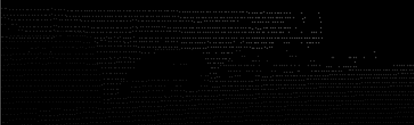
\includegraphics[width=0.46\textwidth]{pics/kitti_cropped.png}
	\caption{Example fromm depth\_data\_velodyne\cite{kitti_dataset}}
	\label{Pic1}
\end{figure}

\paragraph{Rendered Images}
In addition to depth images, attempts were made to use rendered images. However, there appears to be an issue with the file type, which prevents feature detection from being performed. As a result, the program only initializes and then terminates.

\paragraph{Flexion Images}
Another test run was conducted using Flexion Images. These Flexion Images are derived from the original depth images and are merely a further processed version of them. With these images, the entire program ran successfully, meaning that both features and matches were found, and these were then used for pose reconstruction.

\begin{figure}[h]
	\centering
	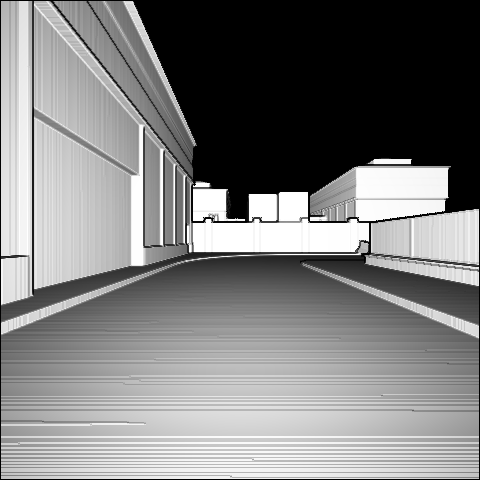
\includegraphics[width=0.46\textwidth]{pics/flexion.png}
	\caption{Example of an Flexion Image}
	\label{Pic2}
\end{figure}

\paragraph{Hardware and Software Constraints}
The evaluation of the benchmarks was performed on a 12-core (i7-8750H) laptop with 64GB RAM and the integrated GPU (iGPU). The calculation of the pose, features, and matchings was done solely on the CPU. No GPU acceleration was used. It is assumed that an implementation utilizing the GPU would achieve significantly higher performance.

\paragraph{Limitations of OpenCV Implementation}
The non-proprietary implementation of OpenCV was used, which limits the selection of feature detection algorithms. The methods used for feature detection and matching were SIFT, ORB, and AKAZE, as these are well-supported by OpenCV and provide a good balance between accuracy and computational efficiency.

\paragraph{Evaluation Metrics}
The evaluation metrics for the benchmarks include the time taken for pose reconstruction, the cumulative deviation from the original path in the X, Y, and Z directions, and the minimum, maximum, and average errors in the three directions. These metrics provide a comprehensive assessment of the performance of the pose estimation algorithms.

\section{Benchmark Description}
The benchmark involves evaluating the performance of the SIFT, ORB, and AKAZE algorithms in terms of pose estimation accuracy and computational efficiency. The depth images as well as the flexion images used in this study were generated from a Blender map using the "blainder" plugin and a self-implemented tool for converting depth images into flexion images. The evaluation metrics include the time taken for pose reconstruction/estimation per image and for the complete data set, the cumulative deviation from the original path in the X, Y, and Z directions, and the minimum, maximum, and average errors in the three directions.

The tests were conducted with a fully charged battery and the computer connected to the power supply. The power mode was set to "Performance" to ensure maximum possible performance. This is important because some laptops tend to throttle CPU performance when running on battery power. Additionally, all other applications were closed during the tests to allow the feature detection and matching program with pose estimation to utilize all available resources.

The tests were performed using both the dataset of depth images and the dataset of flexion images. The FLANN algorithm was used for matching the descriptors in each test. For each test run, both the descriptor and detector algorithms were identical (i.e., SIFT, ORB, and AKAZE). After each test, a pause of approximately 5 minutes was taken to allow the device to cool down, preventing potential thermal throttling at the start of a new test. A total of six tests were conducted: three for depth images with SIFT, AKAZE, and ORB, and three for flexion images with SIFT, AKAZE, and ORB.

For all six tests, the output/writing of the descriptors and keypoints as text files and the generation of matchings as side-by-side images with corresponding markings using colored lines between the keypoints of the two images were disabled.

The detailed procedure for conducting the tests is as follows:
\begin{enumerate}
	\item \textbf{Preparation:} Ensure the laptop is fully charged and connected to the power supply. Set the power mode to "Performance" and close all other applications.
	\item \textbf{Dataset Selection:} Select the dataset to be used (either depth images or flexion images).
	\item \textbf{Algorithm Selection:} Choose the feature detection and matching algorithm (SIFT, ORB, or AKAZE).
	\item \textbf{FLANN Matching:} Use the FLANN algorithm to match the descriptors. Note that FLANN is used for matching descriptors, not keypoints.
	\item \textbf{Pose Estimation:} Run the pose estimation algorithm using the selected dataset and feature detection method. Record the time taken for pose reconstruction/estimation per image and for the complete dataset.
	\item \textbf{Cooling Period:} After each test, allow the laptop to cool down for approximately 5 minutes to prevent thermal throttling.
	\item \textbf{Repeat:} Repeat the above steps for each combination of dataset and feature detection algorithm.
\end{enumerate}

The evaluation metrics for the benchmarks include:

\begin{itemize}
	\item Time taken for pose reconstruction/estimation per image and for the complete dataset.
	\item Cumulative deviation from the original path in the X, Y, and Z directions.
	\item Minimum, maximum, and average errors in the three directions.
\end{itemize}


\subsection{Benchmark Results}

\paragraph{General Expectations}

Under the assumption that the implementation of the pose estimation is correct, similar results in terms of the quality of pose estimation should be expected across all test runs with the corresponding algorithms and input data. Ideally, the absolute path should deviate little to none from the estimated path. Consequently, the representation of the difference between the absolute path and the reconstructed path should approximate the shape of a sphere. This would indicate that the errors/deviations at each data point are within a certain order of magnitude. Thus, the total deviation should be within a certain order of magnitude for all three directions. If a different shape emerges, it suggests that errors in a particular direction or rotational axis are larger.

Under this assumption, the cumulative error in all directions should grow, but only because it consists of the absolute values of the deviations between the estimation and the absolute position. Both the minimum, maximum, and average deviations of each axis should be within a similar order of magnitude. Additionally, these deviations for each axis should be within a similar order of magnitude. Otherwise, it could indicate that the reconstruction/pose estimation is not as reliable/stable in certain directions as in others.

The actual results, unfortunately, do not meet the expectations.
\subsection{Results}
\paragraph{SIFT}
The SIFT algorithm showed the following results:

\begin{itemize}
	\item Fastest processing time: Depth images
	\item Slowest processing time: Flexion images
	\item Lowest cumulative error: Depth images
	\item Highest cumulative error: Flexion images
\end{itemize}

The SIFT algorithm performed better with depth images compared to flexion images. The processing times were faster, and the cumulative errors were lower for depth images. This suggests that SIFT is in this case more efficient and accurate when working with depth images.

\paragraph{AKAZE}
The AKAZE algorithm showed the following results:

\begin{itemize}
	\item Fastest processing time: Depth images
	\item Slowest processing time: Flexion images
	\item Lowest cumulative error: Depth images
	\item Highest cumulative error: Flexion images
\end{itemize}

Similar to SIFT, the AKAZE algorithm performed better with depth images. The processing times were faster, and the cumulative errors were lower for depth images. This indicates that AKAZE is in this case more efficient and accurate with depth images.

\paragraph{ORB}
The ORB algorithm showed the following results:

\begin{itemize}
	\item Fastest processing time: Depth images
	\item Slowest processing time: Flexion images
	\item Lowest cumulative error: Depth images
	\item Highest cumulative error: Flexion images
\end{itemize}

The ORB algorithm also performed better with depth images. The processing times were the fastest among the three algorithms, and the cumulative errors were lower for depth images. This suggests that ORB is highly efficient and more accurate with depth images.

\subsubsection{Overall Comparison}
When comparing all three algorithms and both datasets, the following observations can be made:

\begin{itemize}
	\item Fastest Algorithm: ORB with depth images
	\item Slowest Algorithm: SIFT with flexion images
	\item Lowest Cumulative Error: SIFT with depth images
	\item Highest Cumulative Error: AKAZE with flexion images
	\item Highest Maximum Error: AKAZE with flexion images
\end{itemize}

\begin{figure}[h]
	\centering
	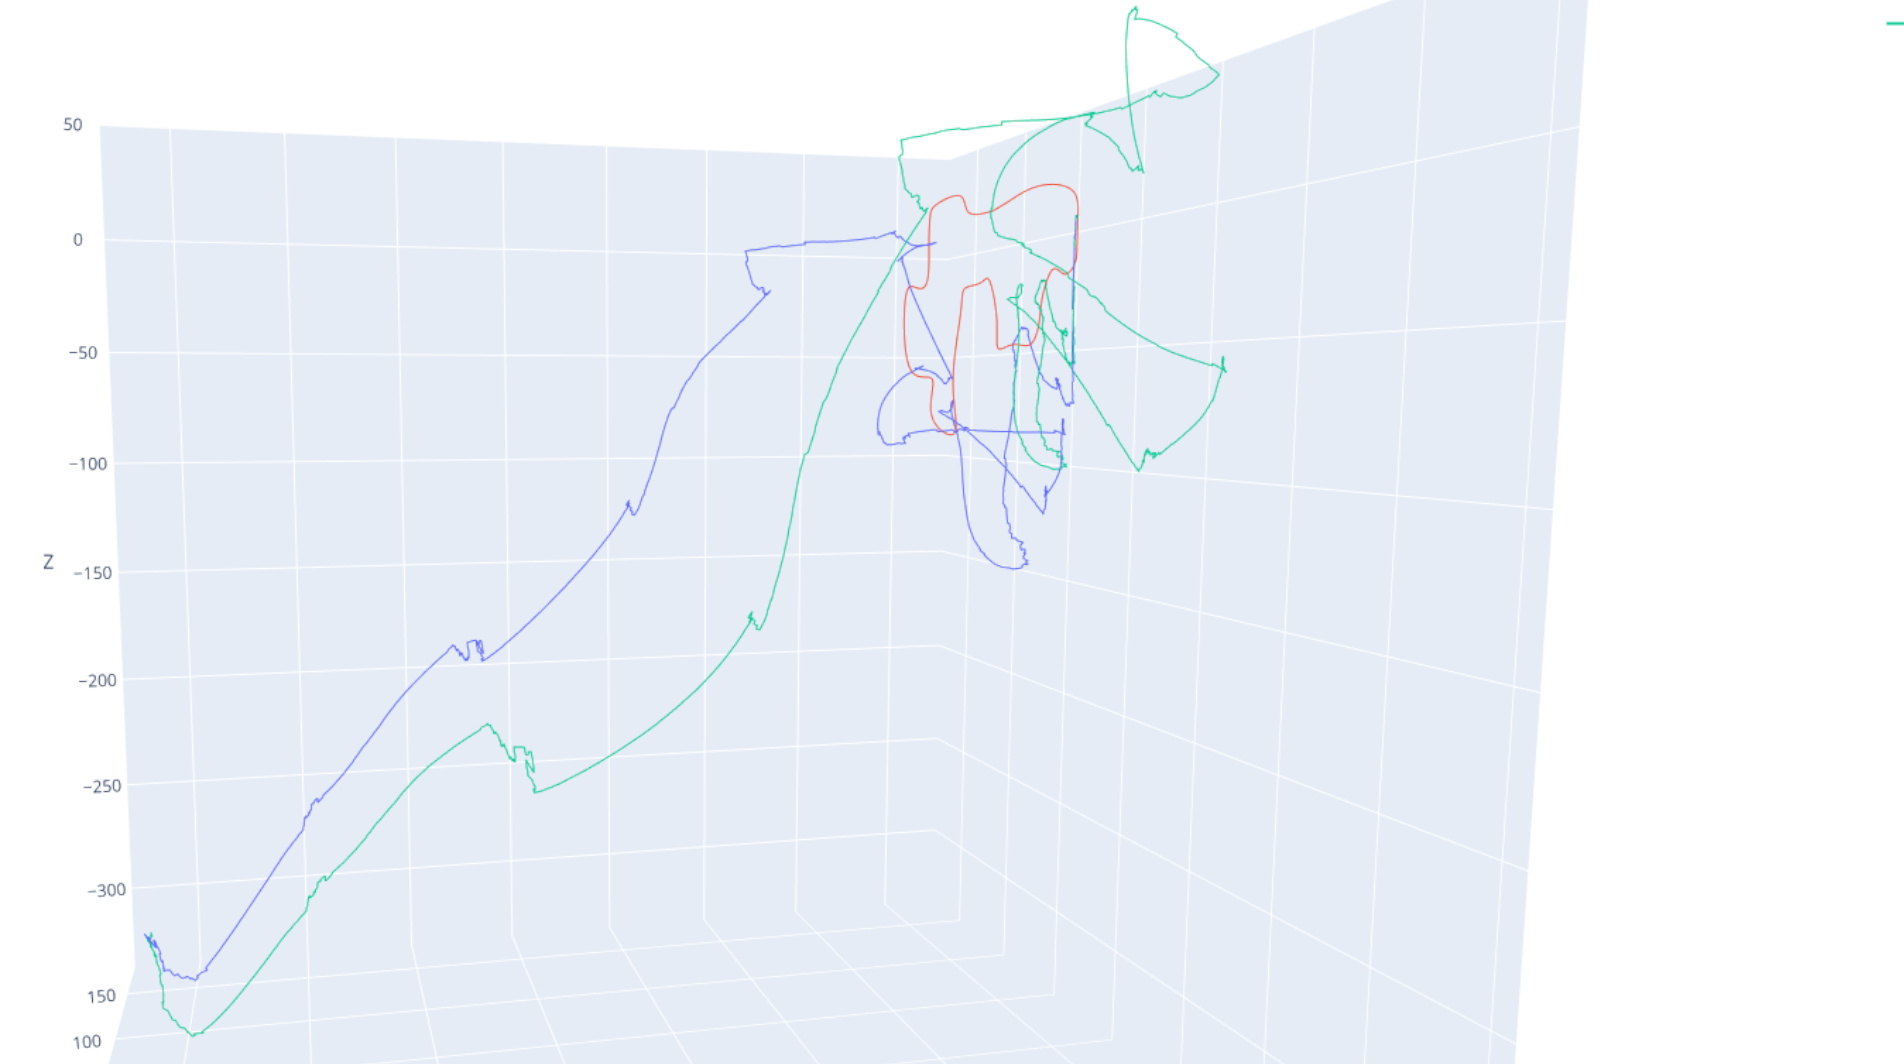
\includegraphics[width=0.6\textwidth]{pics/newplot.png}
	\caption{Interactive Plot of Pose Estimation with SIFT and Flexion Images, red: ground truth, blue: pose estimation, green: difference}
	\label{Pic3}
\end{figure}
There is a significant difference between the use of flexion images and depth images. All three algorithms performed better with depth images in terms of processing time and cumulative error. The flexion images resulted in higher cumulative errors and longer processing times, indicating that depth images are more suitable for pose estimation tasks, at least with this implementation of the feature detection, matching and pose estimation.

\begin{table}[]
	\label{tab1}
	\begin{center}
		\begin{tabular}{llll}
			Image processing time (FPS) & SIFT & AKAZE & ORB   \\
			depth images:               &      &       &       \\
			min                         & 2.13 & 2.67  & 2.63  \\
			max                         & 5.57 & 7.10  & 12.76 \\
			avg                         & 3.87 & 4.62  & 7.68  \\
			flexion images:             &      &       &       \\
			min                         & 1.80 & 2.31  & 2.49  \\
			max                         & 4.08 & 4.90  & 8.30  \\
			avg                         & 2.51 & 3.29  & 5.05 
		\end{tabular}
		\caption{Table of processing times per algorithm and data set.}
	\end{center}
\end{table}
The exact results in terms of processing time can be found in the table \ref{tab1}. 

Upon examining the magnitude of the errors, it is evident that the cumulative errors in all scenarios are substantial. The interactive graphics of the test runs suggest that these errors might be due to incorrect orientation alignment. During the implementation, all possible combinations of rotations and reference axes were tested, including a general offset of the rotation. In none of the tested configurations could the pose estimation be aligned with the absolute path. This indicates an implementation error. Regardless, if the quality of the pose reconstruction were adequate, there should at least be a visual similarity. This is not the case. In some test runs, "knots" appear, indicating that the algorithm detected abrupt changes in direction at these points. However, when examining the matchings, no significant errors are apparent. Although matchings are occasionally incorrect, the majority of matchings in each image pair are correct within a range that would result in small deviations in pose estimation, but not to the extent observed. Notably, in all test scenarios, the flexion images appear more stable and contain fewer of these "knots" when viewed in the interactive plots.

In summary, the comparison has limited significance. The performance is insufficient for real-time applications. It is likely due to the Python implementation and the lack of graphics acceleration. The interactive plots also indicate that flexion images result in more stable pose estimations than pure depth images. To obtain more meaningful results, the pose reconstruction function needs to be revised. It is likely that there was some form of misalignment of the axes and rotations. 

It should also be noted that using flexion images requires preprocessing the respective depth image, which consumes computation time. With the implementation used here, real-time capability is far from being achieved\cite{fleischer}.

All results, test data, and the tool can be found in the repository \cite{repo1}.


\section{Conclusion}

In this study, various test runs were conducted using different datasets. Unfortunately, the results did not meet expectations, which appears to be solely due to the implementation of the pose estimation. It can be assumed that the cause is the swapping of data for the respective axes and rotations. This issue could not be resolved by the time the work was completed. Consequently, the results of the feature-based pose estimation do not show any resemblance to the ground truth. However, this seems to be merely a methodological problem of the implementation.

Regardless, it is evident that there are differences between the types of datasets used. The flexion images show a significantly more stable path compared to the normal depth images. Therefore, it can be assumed that these are advantageous for more accurate pose estimation, but only under the condition that a real-time capable implementation for the calculation of these flexion images is used, as in \cite{toth}. In all cases, real-time capability cannot be achieved, as all tested algorithms with the specific implementation only reached frame rates in the low double-digit range.

Future work could focus on revising the existing framework to ensure that pose estimation or orientation works reliably. For practical applications, it would also be essential to improve the performance of the implementation. This could be achieved by using graphics acceleration or by using hardware-near programming languages such as C++. If the approach of flexion images is further pursued, it would also be necessary to integrate this calculation into the process chain.


\bibliographystyle{IEEEtran}
\bibliography{cite.bib}

\end{document}


